\DocumentMetadata{testphase = {phase-II,sec,toc,graphic,minipage,text}}
\documentclass[a4paper]{article}


% Fonts
\usepackage[T1]{fontenc} % encoding
\renewcommand{\familydefault}{\sfdefault} % sans-serif
\usepackage[nopatch=footnote]{microtype} % better font looking


% Add \extra info to title
\makeatletter
\providecommand{\extra}[1]{
  \apptocmd{\@author}{
    \end{tabular}
    \par\vspace*{0.7em}
    \begin{tabular}[t]{c}
    #1}{}{}
}
\makeatother


% Code integration
\usepackage{minted}
\setminted[c]{autogobble,frame=lines} % code
\setminted[ada]{autogobble}           % stats de vol
\usemintedstyle{emacs}


% Langages
\usepackage[french]{babel}
\frenchsetup{SmallCapsFigTabCaptions=false}
\usepackage{csquotes}
\MakeOuterQuote{"}


% Aliases
\def\coeur{c\oe{}ur}
\def\mone{\textit{Machine 1}} % fixe
\def\mtwo{\textit{Machine 2}} % portable
\def\qs{\enquote{quicksort}}
\def\mandel{\enquote{mandelbrot}}
\def\bone{\textit{Benchmark \qs}}
\def\btwo{\textit{Benchmark \mandel}}
\def\ws{\enquote{work-stealing}}


% Plots
\usepackage{pgfplots}
\pgfplotsset{compat=1.11}


% Images
\usepackage{graphicx}
\usepackage{caption}
\captionsetup{justification=centering}


% Metadatas
\def\titleName{Projet : Un ordonnanceur par work-stealing}
\def\docTitle{\href{https://www.irif.fr/~jch/enseignement/systeme/projet.pdf}{\titleName}}

\def\anri{Anri Kennel}
\def\authorMail{mailto:anri.kennel@etu.u-paris.fr}
\def\docSubject{Programmation système avancée}
\def\docLocation{Université Paris Cité}

\usepackage[
  pdfauthor={\anri},        % author  metadata
  pdftitle={\titleName},    % title   metadata
  pdfsubject={\docSubject}, % subject metadata
  hidelinks,                % clickable links in table of contents
]{hyperref}

\title{\docTitle}
\author{\href{\authorMail}{\anri}\thanks{\anri : 22302653}}
\extra{\docSubject~$\cdot$ \docLocation}
\date{Année universitaire 2023-2024}


% Commands
\newcommand{\docref}[1]{\textit{\nameref{#1}}} % italic nameref
\newcommand{\statPlot}[2]{ % plot for stats
  \begin{figure}[H]
    \def\side{0.5\textwidth}
    \def\width{\textwidth}
    \def\height{0.7\textwidth}
    \def\xlabel{Itérations}
    \def\ylabel{Secondes}
    \def\colname{#1}

    \begin{minipage}{\side}
      \centering
      \begin{tikzpicture}
        \begin{axis}[
            xlabel={\xlabel},
            ylabel={\ylabel},
            width=\width,
            height=\height
          ]
          \addplot [smooth, color=red] table [
              x expr=\coordindex,
              y=\colname,
              col sep=semicolon,
              /pgf/number format/read comma as period] {data/machine1-quicksort.csv};

          \addplot [smooth, color=blue] table [
              x expr=\coordindex,
              y=\colname,
              col sep=semicolon,
              /pgf/number format/read comma as period] {data/machine2-quicksort.csv};
        \end{axis}
      \end{tikzpicture}
      \caption{Temps d'exécution pour \bone~\textit{#2}}
    \end{minipage}\hfill
    \begin{minipage}{\side}
      \centering
      \begin{tikzpicture}
        \begin{axis}[
            xlabel={\xlabel},
            ylabel={\ylabel},
            legend pos=outer north east,
            width=\width,
            height=\height
          ]
          \addplot [smooth, color=red] table [
              x expr=\coordindex,
              y=\colname,
              col sep=semicolon,
              /pgf/number format/read comma as period] {data/machine1-mandelbrot.csv};
          \addlegendentry{\mone}

          \addplot [smooth, color=blue] table [
              x expr=\coordindex,
              y=\colname,
              col sep=semicolon,
              /pgf/number format/read comma as period] {data/machine2-mandelbrot.csv};
          \addlegendentry{\mtwo}
        \end{axis}
      \end{tikzpicture}
      \caption{Temps d'exécution pour \btwo~\textit{#2}}
    \end{minipage}
  \end{figure}
}

\begin{document}
\maketitle
\flushbottom
\tableofcontents
\clearpage


\section{Descriptions}
Description des différents algorithmes implémentés.

\subsection{Séquentiel}\label{desc:seq}
Cette implémentation lance les tâches sur un \coeur.

\subsection{Threads sans gestion}\label{desc:threads}
Cette implémentation correspond à simplement démarrer un nouveau thread
pour chaque nouvelle tâche.

\subsection{Threads avec pile}\label{desc:th_pile}
Pour cette implémentation, nous gardons en mémoire une pile et nous démarrons
un nombre fixe de threads, et à chaque ajout d'une tâche, le thread l'empile.
Chaque thread récupère la dernière tâche ajoutée à la pile.

\subsubsection{Sélection aléatoire de tâche}
Même fonctionnement que dans l'algorithme de \docref{desc:th_pile}, sauf
qu'au lieu de récupérer la dernière tâche, le thread récupère une tâche
aléatoire de la pile.

\subsection{Répartition par \ws}\label{desc:ws}
Ici, chaque \coeur~a sa propre liste de tâches. Quand un thread n'a
plus de tâches, il essaie d'en voler une à un autre thread.


\section{Comportement}

Analyse du comportement des différentes implémentations.

\subsection{Threads sans gestion}
Cette implémentation n'ordonnance rien, alors le nombre de threads
créés est important.

\subsection{Listes}
Dans l'ordonnanceur LIFO, la liste est une pile. Chaque thread récupère le
premier élément de la pile, c'est-à-dire le dernier à avoir été ajouté.

Avec la répartition par \ws, la liste est une deque. Comme dans l'ordonnanceur
LIFO, chaque thread récupère le premier élément de la deque, mais quand il y a
un vol, c'est le dernier élément qui est récupéré par le thread.

\subsection{Synchronisations}
Dans mes implémentations, j'ai exclusivement utilisé des mutex ainsi que des
variables de conditions pour endormir/réveiller mes threads.

Pendant le développement, j'ai parfois utilisé \texttt{usleep} pour interrompre
à temps donné un thread au lieu des variables de conditions pour faire
attendre les threads, mais j'ai obtenu de meilleurs résultats avec les variables
de conditions. Aussi, je pense qu'avoir les variables de conditions m'assure
que mon ordonnanceur fonctionne sur n'importe quel CPU, qu'il soit lent ou rapide,
avec des performances honnêtes. En effet, choisir une valeur qui fonctionne bien
sur mon ordinateur n'assure pas qu'elle soit la meilleure pour un autre processeur.

\subsection{Nombre de threads}
Pour avoir un programme performant, il faut équilibrer le nombre de threads par
rapport aux nombres de \coeur{}s disponibles. Il faut également équilibrer la
création de nouvelles tâches par thread par rapport au véritable travail
effectué par ledit thread. Par exemple, dans le \btwo, chaque tâche crée soit
quatre nouvelles tâches, soit calcule une portion de l'image. Une plus grande
création de tâches favorise le \ws~parce qu'une pile unique atteint ses limites
quand trop de tâches sont ajoutées, car les threads n'ont pas le temps
"d'abattre le travail" assez rapidement.


\section{Statistiques}\label{sec:stats}

Chaque implémentation a été testée avec l'optimisation de niveau 2
de \texttt{gcc}, sur 2 machines.

\begin{enumerate}
  \item \textbf{12 \coeur{}s} pour la \mone.
  \item \textbf{8 \coeur{}s} pour la \mtwo.
\end{enumerate}

Les benchmarks utilisés pour tester les implémentations sont le \qs~fourni
et une adaptation de \mandel~fournie dans le
\href{https://www.irif.fr/~jch/enseignement/systeme/tp10.pdf}{TP 10}.

Pour lancer plusieurs fois le programme, j'ai utilisé la commande
\mintinline{fish}|for| du shell \texttt{fish}. Pour exemple, voici la commande
pour lancer l'ordonnanceur 100 fois avec \qs~et tous les threads disponibles :

\begin{figure}[H]
  \centering
  \mintinline{fish}|for i in (seq 100); ./ordonnanceur.elf -qt 0; end|
\end{figure}

\subsection{Séquentiel}\label{stats:seq}
\begin{description}
  \item[\bone] \hspace{1em}
        \begin{description}
          \item[\mone] Le programme a été lancé \textbf{100 fois}.
                Le temps moyen d'exécution a été de \textbf{0,855 secs}
          \item[\mtwo] Le programme a été lancé \textbf{100 fois}.
                Le temps moyen d'exécution a été de \textbf{1,139 secs}
        \end{description}

  \item[\btwo] \hspace{1em}
        \begin{description}
          \item[\mone] Le programme a été lancé \textbf{10 fois}.
                Le temps moyen d'exécution a été de \textbf{3,733 secs}
          \item[\mtwo] Le programme a été lancé \textbf{10 fois}.
                Le temps moyen d'exécution a été de \textbf{6,020 secs}
        \end{description}
\end{description}

\statPlot{serial}{en séquentiel}

\begin{figure}[H]
  \centering
  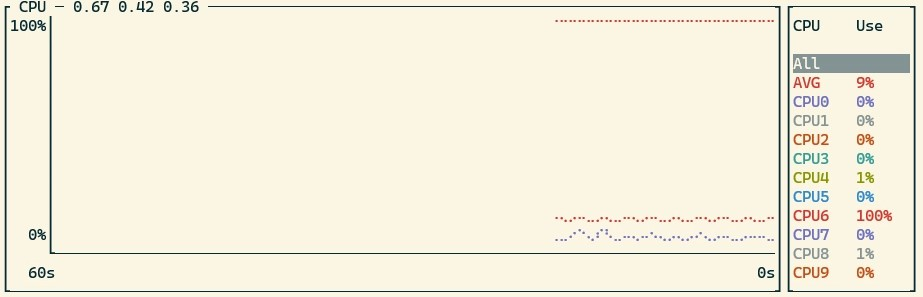
\includegraphics[alt={Graphique},width=\textwidth]{imgs/bottom-seq.jpg}
  \caption{Exploitation des ressources sur la \mone~avec \docref{desc:seq}}
  \label{fig:btm-seq}
\end{figure}

Ce programme ne bénéficie pas de toute la puissance de la machine,
visible notamment grâce à la \autoref{fig:btm-seq} où l'on voit que seulement
un \coeur~est utilisé.

\subsection{Threads sans gestion}\label{stats:th_ges}

\begin{description}
  \item[\bone] \hspace{1em}
        \begin{description}
          \item[\mone] Le programme a été lancé \textbf{10 fois}.
                Le temps moyen d'exécution a été de \textbf{35,985 secs}
          \item[\mtwo] Le programme a été lancé \textbf{10 fois}.
                Le temps moyen d'exécution a été de \textbf{18,854 secs}
        \end{description}

  \item[\btwo] \hspace{1em}
        \begin{description}
          \item[\mone] Le programme a été lancé \textbf{10 fois}.
                Le temps moyen d'exécution a été de \textbf{66,078 secs}
          \item[\mtwo] Le programme a été lancé \textbf{10 fois}.
                Le temps moyen d'exécution a été de \textbf{41,060 secs}
        \end{description}
\end{description}

\statPlot{solution1}{avec des threads}

\begin{figure}[H]
  \centering
  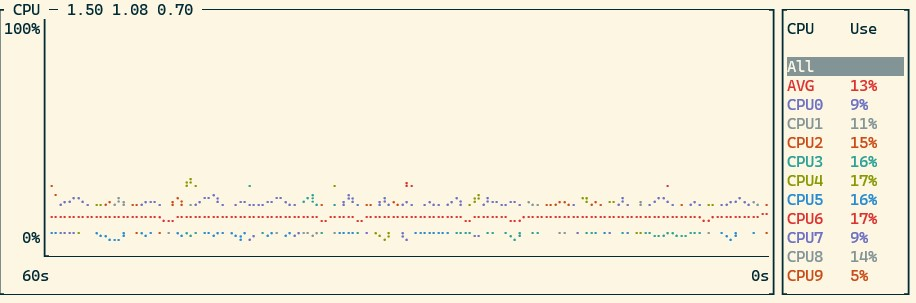
\includegraphics[alt={Graphique},width=\textwidth]{imgs/bottom-threads.jpg}
  \caption{Exploitation des ressources sur la \mone~avec \docref{desc:threads}}
  \label{fig:btm-threads}
\end{figure}

La création des threads pour chaque tâche crée un énorme goulot
d'étranglement qui réduit grandement les performances. On le voit notamment
sur la \autoref{fig:btm-threads} où tous les \coeur{}s sont utilisés, mais très
peu. Créer de façon incontrôlée des threads n'est pas une manière efficace de
répartir la charge.

% Le temps d'exécution étant long, nous pouvons voir les threads avec la commande
% \texttt{top} : \mintinline{bash}|top -Hp $(pgrep ordonnanceur)|.

Pour augmenter les performances, il faut donc avoir une taille fixe de threads,
et par conséquent, il faut gérer les tâches et décider de quelle tâche va sur
quel thread.

\subsection{Threads avec pile}\label{stats:stack}
\begin{description}
  \item[\bone] \hspace{1em}
        \begin{description}
          \item[\mone] Le programme a été lancé \textbf{100 fois}.
                Le temps moyen d'exécution a été de \textbf{0,258 secs}
          \item[\mtwo] Le programme a été lancé \textbf{100 fois}.
                Le temps moyen d'exécution a été de \textbf{0,356 secs}
        \end{description}

  \item[\btwo] \hspace{1em}
        \begin{description}
          \item[\mone] Le programme a été lancé \textbf{100 fois}.
                Le temps moyen d'exécution a été de \textbf{0,787 secs}
          \item[\mtwo] Le programme a été lancé \textbf{100 fois}.
                Le temps moyen d'exécution a été de \textbf{1,858 secs}
        \end{description}
\end{description}

\statPlot{solution2}{avec LIFO}

Le lancement de nouveaux threads étant limité, les performances
sont grandement améliorées par rapport aux tests de \docref{stats:th_ges}.

Également, grâce au fait que désormais nous utilisons les \coeur{}s~de notre CPU,
les performances sont aussi améliorées par rapport aux tests de
\docref{stats:seq}.

Dans la \autoref{fig:btm-lifo}, nous observons que les \coeur{}s du CPU ne sont pas
tous utilisés à 100~\%. Ceci est dû au fait que l'accès à la liste des tâches est
limité, car partagé entre les threads.

\begin{figure}[H]
  \centering
  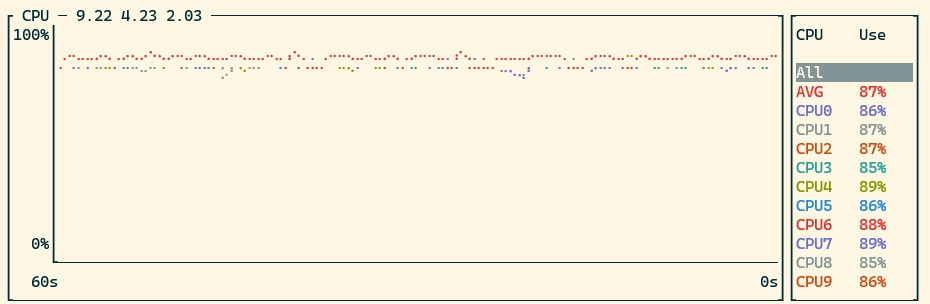
\includegraphics[alt={Graphique},width=\textwidth]{imgs/bottom-lifo.jpg}
  \caption{Utilisation ressources sur la \mone~avec \docref{desc:th_pile}}
  \label{fig:btm-lifo}
\end{figure}

\subsubsection{Sélection aléatoire de tâche}
\begin{description}
  \item[\bone] \hspace{1em}
        \begin{description}
          \item[\mone] Le programme a été lancé \textbf{100 fois}.
                Le temps moyen d'exécution a été de \textbf{0,390 secs}
          \item[\mtwo] Le programme a été lancé \textbf{100 fois}.
                Le temps moyen d'exécution a été de \textbf{0,438 secs}
        \end{description}

  \item[\btwo] \hspace{1em}
        \begin{description}
          \item[\mone] Le programme a été lancé \textbf{100 fois}.
                Le temps moyen d'exécution a été de \textbf{0,438 secs}
          \item[\mtwo] Le programme a été lancé \textbf{100 fois}.
                Le temps moyen d'exécution a été de \textbf{1,887 secs}
        \end{description}
\end{description}

\statPlot{solution3}{avec LIFO aléatoire}

Cette implémentation est identique à \docref{stats:stack}, à l'exception que
les threads récupèrent une tâche aléatoire de la pile au lieu d'y prendre
la dernière ajoutée.

Cette façon de faire réduit les performances.

\subsection{Répartition par \ws}
\begin{description}
  \item[\bone] \hspace{1em}
        \begin{description}
          \item[\mone] Le programme a été lancé \textbf{100 fois}.
                Le temps moyen d'exécution a été de \textbf{0,229 secs}
          \item[\mtwo] Le programme a été lancé \textbf{100 fois}.
                Le temps moyen d'exécution a été de \textbf{0,308 secs}
        \end{description}

  \item[\btwo] \hspace{1em}
        \begin{description}
          \item[\mone] Le programme a été lancé \textbf{100 fois}.
                Le temps moyen d'exécution a été de \textbf{0,447 secs}
          \item[\mtwo] Le programme a été lancé \textbf{100 fois}.
                Le temps moyen d'exécution a été de \textbf{1,131 secs}
        \end{description}
\end{description}

\statPlot{solution4}{avec du \ws}

Dans cette implémentation, nous n'utilisons plus une pile, mais un deque de tâches.
Cette façon de faire est légèrement meilleur que \docref{desc:th_pile}.

Dans la \autoref{fig:btm-ws}, nous observons que les \coeur{}s du CPU sont
proches de 100~\% d'utilisation. Comparé à \docref{stats:stack}, nous gagnons
en moyenne \approx~10~\% de l'utilisation du processeur dans son entièreté.

\begin{figure}[H]
  \centering
  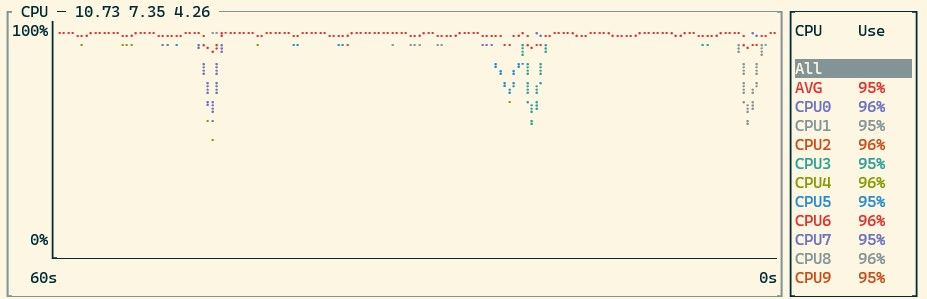
\includegraphics[alt={Graphique},width=\textwidth]{imgs/bottom-ws.jpg}
  \caption{Exploitation des ressources sur la \mone~avec \docref{desc:ws}}
  \label{fig:btm-ws}
\end{figure}

Concernant les statistiques de vols, les résultats sont obtenus en récupérant
les données par thread en prenant des précautions pour ne pas dégrader les
performances de l'ordonnanceur. Les données sont récoltées par thread et ensuite
tout est additionné quand toutes les tâches sont terminées.

\begin{description}
  \item[\bone] \hspace{1em}
        \begin{description}
          \item[\mone] \hspace{1em}
                \begin{samepage}
                  \begin{minted}{ada}
                    ------- Satistiques -------
                     Total tâches       : 368439
                     Total vols         : 5484
                     Total vols réussis : 5222
                     Total vols échoués : 262
                    ----------------------------
                  \end{minted}
                \end{samepage}
          \item[\mtwo] \hspace{1em}
                \begin{samepage}
                  \begin{minted}{ada}
                    ------- Statistiques -------
                     Total tâches       : 368439
                     Total vols         : 2298
                     Total vols réussis : 2164
                     Total vols échoués : 134
                    ----------------------------
                  \end{minted}
                \end{samepage}
        \end{description}

  \item[\btwo] \hspace{1em}
        \begin{description}
          \item[\mone] \hspace{1em}
                \begin{samepage}
                  \begin{minted}{ada}
                    ------- Statistiques -------
                     Total tâches       : 873813
                     Total vols         : 23232
                     Total vols réussis : 23192
                     Total vols échoués : 40
                    ----------------------------
                  \end{minted}
                \end{samepage}
          \item[\mtwo] \hspace{1em}
                \begin{samepage}
                  \begin{minted}{ada}
                    ------- Statistiques -------
                     Total tâches       : 873813
                     Total vols         : 21491
                     Total vols réussis : 21465
                     Total vols échoués : 26
                    ----------------------------
                  \end{minted}
                \end{samepage}
        \end{description}
\end{description}

Nous pouvons remarquer que moins il y a de vols échoués, meilleur est
le temps d'exécution. Également, le nombre de vols échoués est faible quand
beaucoup de tâches sont créées, car la probabilité qu'un thread ait des tâches
en attente est plus grande.


\section{Interprétation}
En se basant sur les résultats des tests de \docref{sec:stats}, on remarque
que l'algorithme de \ws~est le plus performant dans la \mone~ainsi que dans
la \mtwo. Nous voyons aussi que ce système profite d'un grand nombre de
tâches créées, car le \btwo~créant quatre tâches d'un coup provoque nettement
moins de vol comparé au \bone~qui n'en crée que deux.

\clearpage
\appendix
\section{Crédits}

J'ai utilisé un bout de code de \href{https://expreg.org/amsi/C/}{Farès Belhadj}
d'un TP de L2 pour afficher une image au format \texttt{bmp} afin vérifier que
le \btwo~fonctionnait correctement. Ce qui donne la \autoref{fig:mandelbrot}.

\begin{figure}[H]
  \centering
  
\includegraphics[alt={Fractale \mandel},width=0.7\textwidth]{imgs/mandelbrot.jpg}
  \caption{Example de \mandel}
  \label{fig:mandelbrot}
\end{figure}

Les captures d'écran d'exploitation des ressources ont été prises via le
programme \href{https://github.com/ClementTsang/bottom}{bottom}.

\end{document}
